\documentclass{beamer}
\usepackage{amsmath}
\usepackage[english]{babel} %set language; note: after changing this, you need to delete all auxiliary files to recompile
\usepackage[utf8]{inputenc} %define file encoding; latin1 is the other often used option
\usepackage{csquotes} % provides context sensitive quotation facilities
\usepackage{graphicx} %allows for inserting figures
\usepackage{booktabs} % for table formatting without vertical lines
\usepackage{textcomp} % allow for example using the Euro sign with \texteuro
\usepackage{stackengine}
\usepackage{wasysym}
\usepackage{tikzsymbols}
\usepackage{textcomp}
\newcommand{\bubblethis}[2]{
        \tikz[remember picture,baseline]{\node[anchor=base,inner sep=0,outer sep=0]%
        (#1) {\underline{#1}};\node[overlay,cloud callout,callout relative pointer={(0.2cm,-0.7cm)},%
        aspect=2.5,fill=yellow!90] at ($(#1.north)+(-0.5cm,1.6cm)$) {#2};}%
    }%
\tikzset{face/.style={shape=circle,minimum size=4ex,shading=radial,outer sep=0pt,
        inner color=white!50!yellow,outer color= yellow!70!orange}}
%% Some commands to make the code easier
\newcommand{\emoticon}[1][]{%
  \node[face,#1] (emoticon) {};
  %% The eyes are fixed.
  \draw[fill=white] (-1ex,0ex) ..controls (-0.5ex,0.2ex)and(0.5ex,0.2ex)..
        (1ex,0.0ex) ..controls ( 1.5ex,1.5ex)and( 0.2ex,1.7ex)..
        (0ex,0.4ex) ..controls (-0.2ex,1.7ex)and(-1.5ex,1.5ex)..
        (-1ex,0ex)--cycle;}
\newcommand{\pupils}{
  %% standard pupils
  \fill[shift={(0.5ex,0.5ex)},rotate=80] 
       (0,0) ellipse (0.3ex and 0.15ex);
  \fill[shift={(-0.5ex,0.5ex)},rotate=100] 
       (0,0) ellipse (0.3ex and 0.15ex);}

\newcommand{\emoticonname}[1]{
  \node[below=1ex of emoticon,font=\footnotesize,
        minimum width=4cm]{#1};}
\usepackage{scalerel}
\usetikzlibrary{positioning}
\usepackage{xcolor,amssymb}
\newcommand\dangersignb[1][2ex]{%
  \scaleto{\stackengine{0.3pt}{\scalebox{1.1}[.9]{%
  \color{red}$\blacktriangle$}}{\tiny\bfseries !}{O}{c}{F}{F}{L}}{#1}%
}
\newcommand\dangersignw[1][2ex]{%
  \scaleto{\stackengine{0.3pt}{\scalebox{1.1}[.9]{%
  \color{red}$\blacktriangle$}}{\color{white}\tiny\bfseries !}{O}{c}{F}{F}{L}}{#1}%
}
\usepackage{fontawesome} % Social Icons
\usepackage{epstopdf} % allow embedding eps-figures
\usepackage{tikz} % allows drawing figures
\usepackage{amsmath,amssymb,amsthm} %advanced math facilities
\usepackage{lmodern} %uses font that support italic and bold at the same time
\usepackage{hyperref}
\usepackage{tikz}
\hypersetup{
    colorlinks=true,
    linkcolor=blue,
    filecolor=magenta,      
    urlcolor=blue,
}
\usepackage{tcolorbox}
%add citation management using BibLaTeX
\usepackage[citestyle=authoryear-comp, %define style for citations
    bibstyle=authoryear-comp, %define style for bibliography
    maxbibnames=10, %maximum number of authors displayed in bibliography
    minbibnames=1, %minimum number of authors displayed in bibliography
    maxcitenames=3, %maximum number of authors displayed in citations before using et al.
    minnames=1, %maximum number of authors displayed in citations before using et al.
    datezeros=false, % do not print dates with leading zeros
    date=long, %use long formats for dates
    isbn=false,% show no ISBNs in bibliography (applies only if not a mandatory field)
    url=false,% show no urls in bibliography (applies only if not a mandatory field)
    doi=false, % show no dois in bibliography (applies only if not a mandatory field)
    eprint=false, %show no eprint-field in bibliography (applies only if not a mandatory field)
    backend=biber %use biber as the backend; backend=bibtex is less powerful, but easier to install
    ]{biblatex}
\addbibresource{../mybibfile.bib} %define bib-file located one folder higher


\usefonttheme[onlymath]{serif} %set math font to serif ones

\definecolor{beamerblue}{rgb}{0.2,0.2,0.7} %define beamerblue color for later use

%%% defines highlight command to set text blue
\newcommand{\highlight}[1]{{\color{blue}{#1}}}


%%%%%%% commands defining backup slides so that frame numbering is correct

\newcommand{\backupbegin}{
   \newcounter{framenumberappendix}
   \setcounter{framenumberappendix}{\value{framenumber}}
}
\newcommand{\backupend}{
   \addtocounter{framenumberappendix}{-\value{framenumber}}
   \addtocounter{framenumber}{\value{framenumberappendix}}
}

%%%% end of defining backup slides

%Specify figure caption, see also http://tex.stackexchange.com/questions/155738/caption-package-not-working-with-beamer
\setbeamertemplate{caption}{\insertcaption} %redefines caption to remove label "Figure".
%\setbeamerfont{caption}{size=\scriptsize,shape=\itshape,series=\bfseries} %sets figure  caption bold and italic and makes it smaller


\usetheme{Boadilla}

%set options of hyperref package
\hypersetup{
    bookmarksnumbered=true, %put section numbers in bookmarks
    naturalnames=true, %use LATEX-computed names for links
    citebordercolor={1 1 1}, %color of border around cites, here: white, i.e. invisible
    linkbordercolor={1 1 1}, %color of border around links, here: white, i.e. invisible
    colorlinks=true, %color links
    anchorcolor=black, %set color of anchors
    linkcolor=beamerblue, %set link color to beamer blue
    citecolor=blue, %set cite color to beamer blue
    pdfpagemode=UseThumbs, %set default mode of PDF display
    breaklinks=true, %break long links
    pdfstartpage=1 %start at first page
    }


% --------------------
% Overall information
% --------------------
\title[Principios de Economía]{Principios de Economía}
\date{}
\author[Ertola y Sturzenegger]{Gabriela Ertola y Federico Sturzenegger }
\vspace{0.4cm}
\institute[]{Universidad de San Andrés \\
2022} 


\begin{document}

\begin{frame}
\frametitle{Principios de Economía
\centering
\\ \vspace{12mm} El mercado y sus formas}
\centering
 \\ \vspace{12mm} %5 de agosto, 2021 \vspace{5mm} \\ 

\includegraphics[scale=0.25]{Figures/logoUDESA.jpg} 
\end{frame}


\begin{frame}
\frametitle{¿Se acuerdan del equilibrio de mercado?}
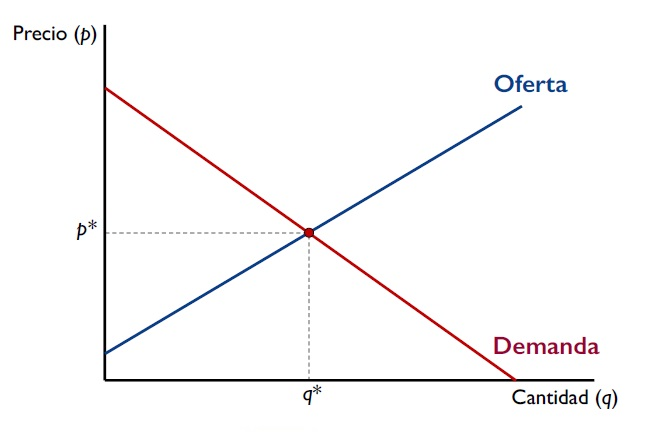
\includegraphics[scale=0.6]{Figures/Tema_07.3_equilibrioofertademanda_0.jpg}
\end{frame}

\begin{frame}
\frametitle{Equilibrio}
\begin{itemize}
    \item En el precio de equilibrio (market-clearing price), la oferta iguala a la demanda
    \item Otros precios no son un equilibrio de Nash
    \begin{itemize}
        \item Si p $>$ p*, entonces habría exceso de oferta \\
        \item Si p $<$ p*, entonces habría exceso de demanda \\
        \item Se asume que los productos son idénticos, por lo que los compradores estarían dispuestos a comprar a cualquier vendedor
    \end{itemize}
\end{itemize}
\end{frame}

\begin{frame}
\frametitle{Competencia y empresas tomadoras de precios}
\begin{itemize}
    \item ¿Cuándo tenemos una mercado competitivo?
    \begin{enumerate}
        \item Muchos compradores y vendedores no diferenciados que actúan en forma independiente
        \item El precio viene determinado por el mercado
        \item Productos ofrecidos básicamente idénticos, y los compradores conocen su precio
        \item Las firmas entran o salen del mercado libremente 
    \end{enumerate}
    \vspace{2mm}
    \item En un mercado competitivo las firmas y los consumidores son tomadores de precios
    \begin{itemize}
        \item Para la firma esto quiere decir que el precio de mercado es igual al ingreso marginal \\
        - ¿Por qué?
    \end{itemize}
\end{itemize}
\end{frame}

\begin{frame}
\frametitle{ Precios determinados por el mercado}
\begin{itemize}
    \item Las firmas son tomadoras de precios, eso quiere decir que no pueden:
    \begin{itemize}
        \item Influir en el precio de mercado
        \item Beneficiarse de la elección de un precio diferente del precio de mercado
    \end{itemize}
    \item La curva de demanda (conjunto factible) de estas firmas se vuelve completamente plana
    \item La curva de oferta es la curva de CMg de la firma
    \end{itemize}
    \begin{center}
        \textbf{La empresa elige cantidad, no precio}
    \end{center}
\end{frame}

\begin{frame}
\frametitle{ ¿Qué pasa en la empresa?}
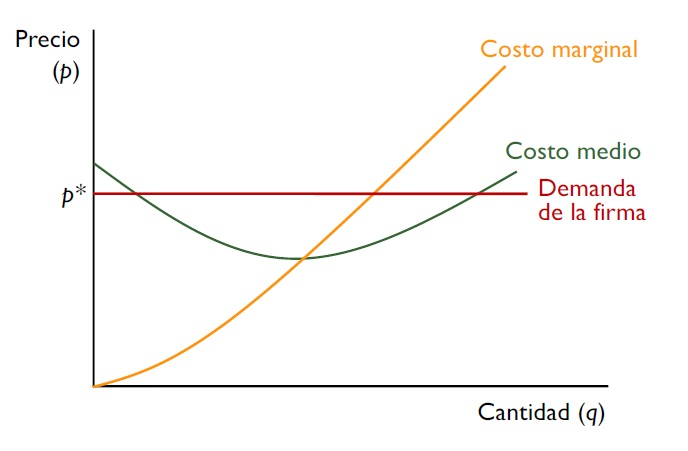
\includegraphics[scale=0.6]{Figures/Tema_07.7_compperfecta.jpg}
\end{frame}

\begin{frame}
\frametitle{ ¿Qué pasa si el precio es mayor que el costo marginal?}
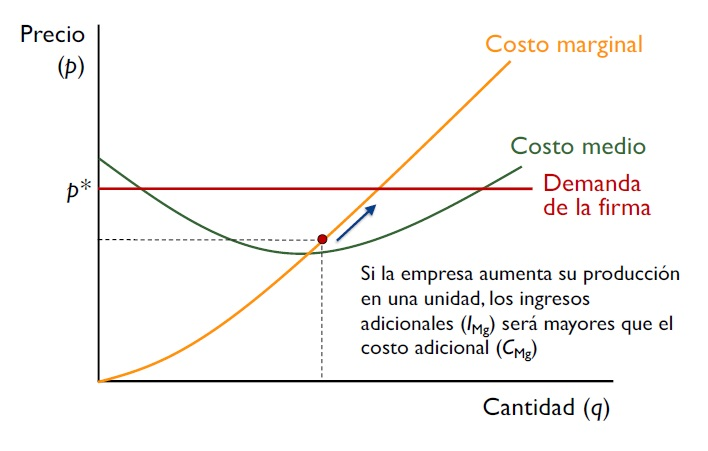
\includegraphics[scale=0.55]{Figures/Tema_07.8_compperfecta2.jpg}
\end{frame}

\begin{frame}
\frametitle{ ¿Qué pasa si el precio es menor que el costo marginal?}
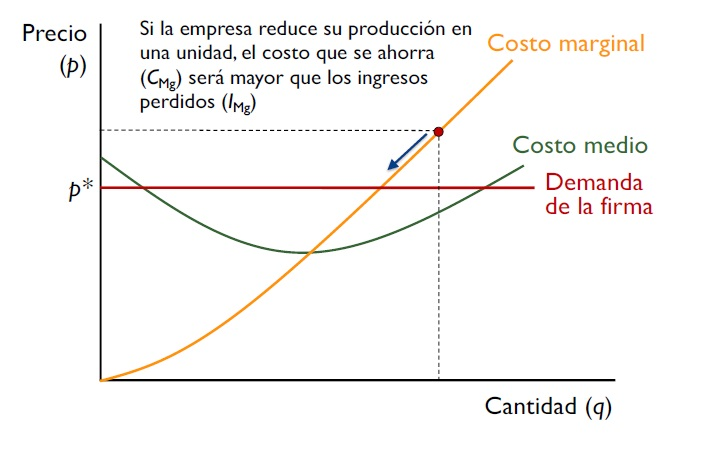
\includegraphics[scale=0.55]{Figures/Tema_07.9_compperfecta3.jpg}
\end{frame}

\begin{frame}
\frametitle{La empresa maximiza beneficios, ¿cómo?}
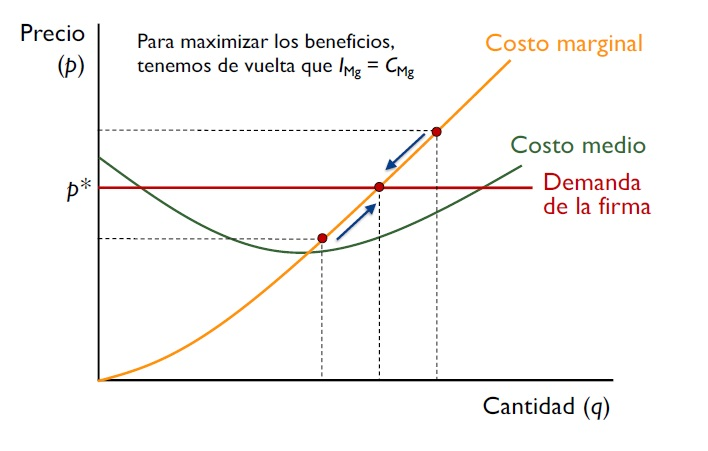
\includegraphics[scale=0.55]{Figures/Tema_07.10_compperfecta4.jpg}
\end{frame}

\begin{frame}
\frametitle{ ¿Habrá beneficio en este punto? SI!}
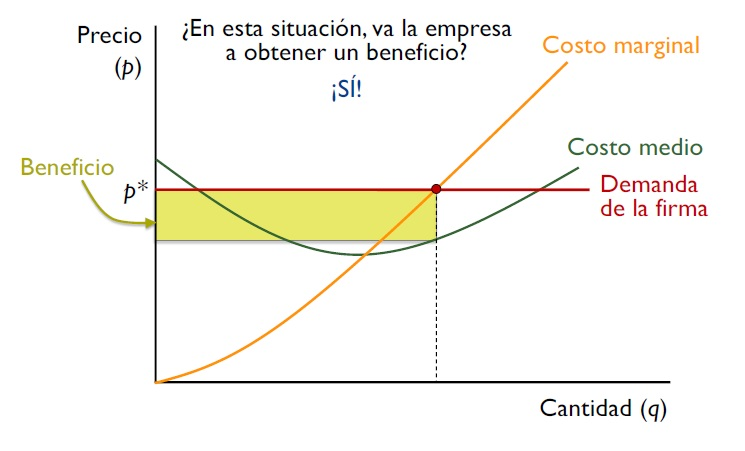
\includegraphics[scale=0.55]{Figures/Tema_07.11_compperfecta5.jpg}
\end{frame}

\begin{frame}
\frametitle{ ¿Habrá beneficio en este punto? NO! ¿Hay perdida? SI!}
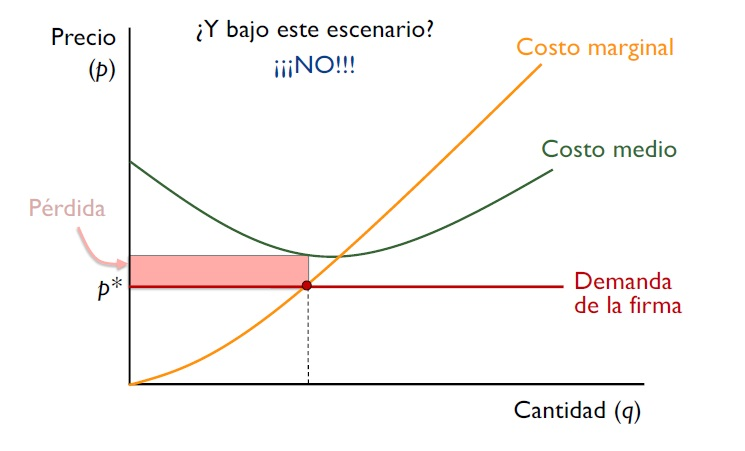
\includegraphics[scale=0.55]{Figures/Tema_07.12_compperfecta6.jpg}
\end{frame}

\begin{frame}
\frametitle{ ¿Habrá beneficio extraordinario en este punto? NO! ¿Hay perdida? NO!}
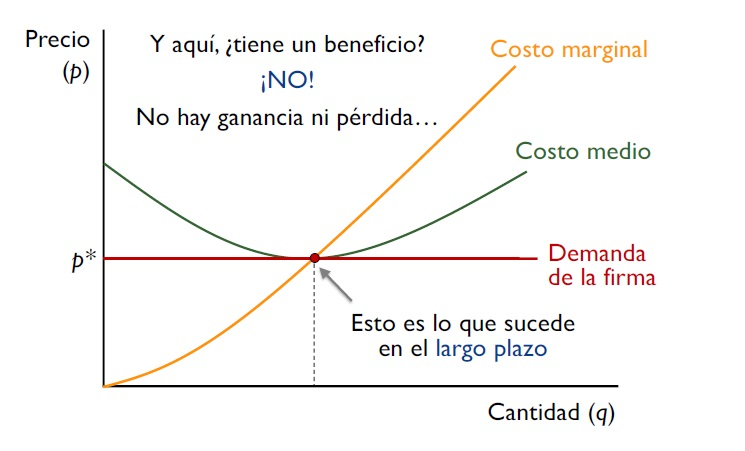
\includegraphics[scale=0.55]{Figures/Tema_07.13_compperfecta7.jpg}
\end{frame}

\begin{frame}
\frametitle{ Beneficios en el largo plazo}
\begin{itemize}
    \item Siempre que existan potenciales rentas (beneficios extraordinarios), va a haber firmas interesadas en entrar al mercado
    \item Si los costos de entrada no son demasiado altos, estas firmas potenciales van a entrar
    \item Al ingresar, las firmas van a presionar hacia abajo el precio de equilibrio, eliminando del mercado a las firmas menos eficientes
    \item Los beneficios que atraen a potenciales entrantes comienzan a disiparse
    \item En el largo plazo, estos beneficios van a desaparecer, serán iguales a 0
    \end{itemize}
\end{frame}

\begin{frame}
\frametitle{Recordemos lo que sucede en equilibrio... beneficios para todos!}
\begin{center}
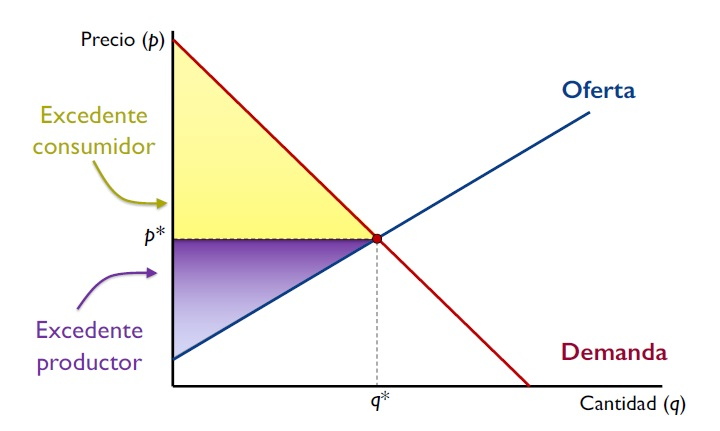
\includegraphics[scale=0.55]{Figures/Tema_07.23_equilibrioyexcedente.jpg}
\end{center}
\end{frame}

\begin{frame}
\frametitle{ ¿Por qué es eficiente?}
\begin{itemize}
    \item Los participantes son tomadores de precios
    \begin{itemize}
        \item No hay poder de mercado
        \item La competencia impide a los vendedores aumentar el precio, y a los compradores bajarlo
    \end{itemize}
    \item Los contratos son completos
        \begin{itemize}
        \item Los detalles del intercambio pueden ser definidos en forma clara, y estos contratos se pueden hacer cumplir
        \end{itemize}
    \item No hay externalidades
        \begin{itemize}
        \item La transacción sólo afecta a los compradores y vendedores
        \end{itemize}
\end{itemize}
\end{frame}


\begin{frame}
\frametitle{El problema de la firma}
\begin{itemize}
    \item Una vez que conocemos la demanda... ¿cómo se elige cuánto producir y el precio que cobrar?
    \vspace{2mm}
    \item El problema principal de la empresa es el de la maximización del beneficio
    \vspace{2mm}     \begin{itemize}
        \item ¿Qué es el beneficio? \vspace{2mm} \\ 
        Beneficio = Ingresos totales – Costos totales
        \vspace{2mm}
        \item ¿Qué es el ingreso total? 
        \vspace{2mm} \\ 
        El valor de la producción al precio ofrecido (p·q)
        \vspace{2mm}
        \item ¿Qué es el costo total?
        \vspace{2mm} \\ 
        Los costos por unidad, por la cantidad de unidades producidas (c·q)
    \end{itemize} 
\end{itemize} 
\end{frame}

\begin{frame}
\frametitle{Monopolios}
\begin{itemize}
    \item Empresa que vende productos especializados tienen un alto poder de mercado
    \begin{itemize}
        \item Enfrentan poca competencia, tienen una demanda inelástica, y pueden fijar precio superior al costo marginal sin perder clientes
        \item Las barreras de entrada ayudan a generar rentas \\
        - Beneficios económicos por encima de los costos de producción
    \end{itemize}
    \item En estos casos, en equilibrio encontramos una pérdida de peso muerto
    \begin{itemize}
        \item Tenemos entonces una falla de mercado \\
        - Es decir, los mercados asignan recursos en una forma
    \end{itemize}
    \end{itemize}
\end{frame}


\begin{frame}
\frametitle{Mirando el ingreso total}
\begin{itemize}
    \item El concepto clave es el de ingreso marginal
    \begin{itemize}
        \item Variación en ingresos al vender una unidad adicional
        \item Efecto neto de la disminución de los precios y el aumento de la cantidad vendida
    \end{itemize}
    \item La curva de demanda nos determina ingresos marginales decrecientes
    \begin{itemize}
        \item ¿Cómo cambia el ingreso al aumentar la producción? \\
        - Ahora se vende una unidad más... \\
        - ...¡pero todas las vendo a un precio menor!
    \end{itemize}
\end{itemize}
\end{frame}

\begin{frame}
\frametitle{ ¿Cómo cambia el ingreso total?}
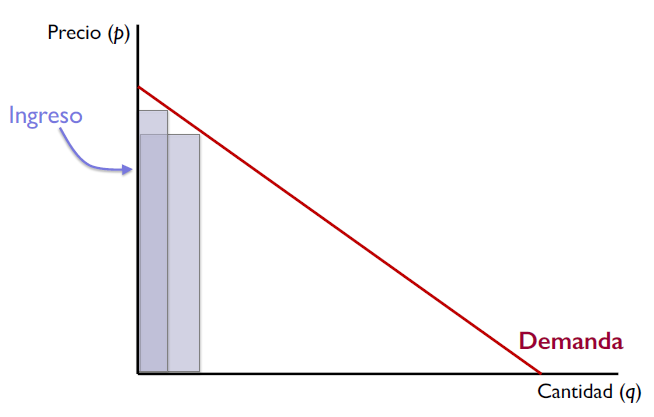
\includegraphics[scale=0.6]{Figures/Tema_06.30_ingresototal.png}
\end{frame}

\begin{frame}
\frametitle{ ¿Cómo cambia el ingreso total?}
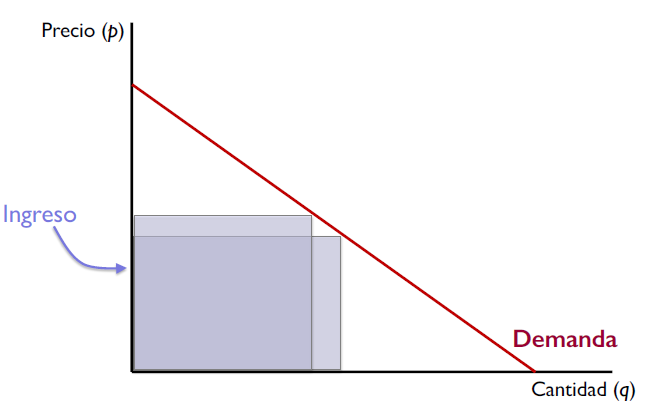
\includegraphics[scale=0.6]{Figures/Tema_06.31_ingresototal2.png}
\end{frame}

\begin{frame}
\frametitle{¿Cómo cambia el ingreso total?}
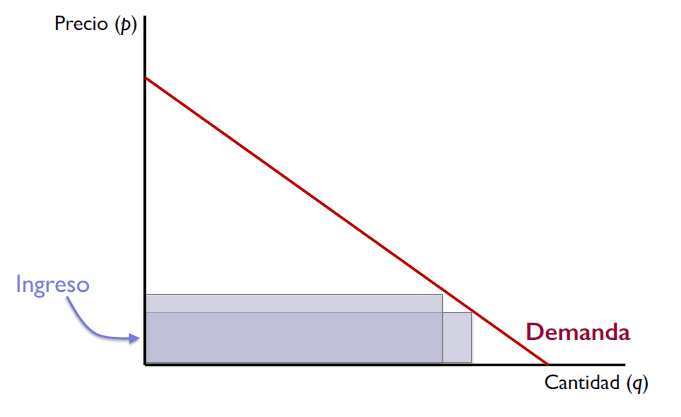
\includegraphics[scale=0.6]{Figures/Tema_06.32_ingresototal3.png}
\end{frame}

\begin{frame}
\frametitle{ El ingreso marginal}
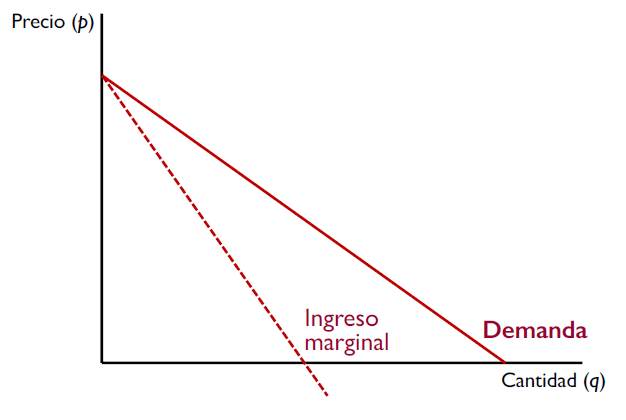
\includegraphics[scale=0.6]{Figures/Tema_06.33_ingresomarginal.png}
\end{frame}

\begin{frame}
\frametitle{ ¿Cómo cambian los beneficios?}
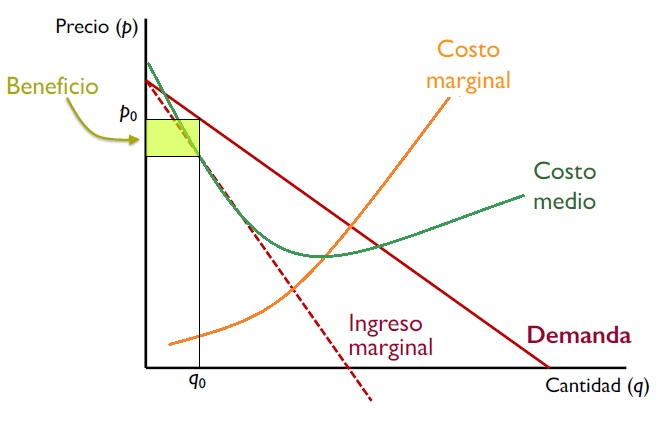
\includegraphics[scale=0.6]{Figures/Tema_06.34_beneficios.jpg}
\end{frame}

\begin{frame}
\frametitle{¿Cómo cambian los beneficios?}
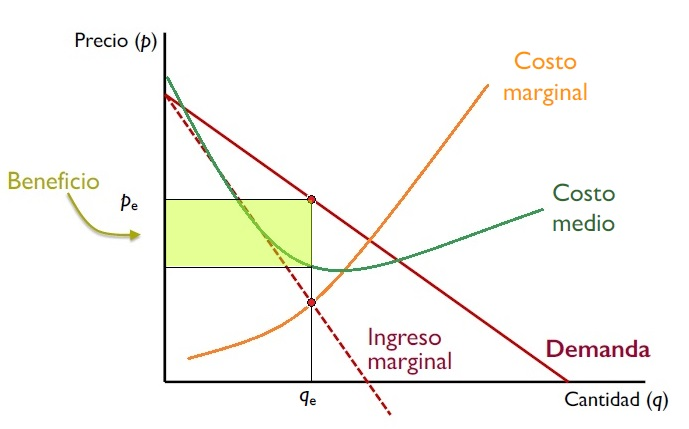
\includegraphics[scale=0.6]{Figures/Tema_06.35_beneficios2.jpg}
\end{frame}

\begin{frame}
\frametitle{ Costo e ingreso marginal}
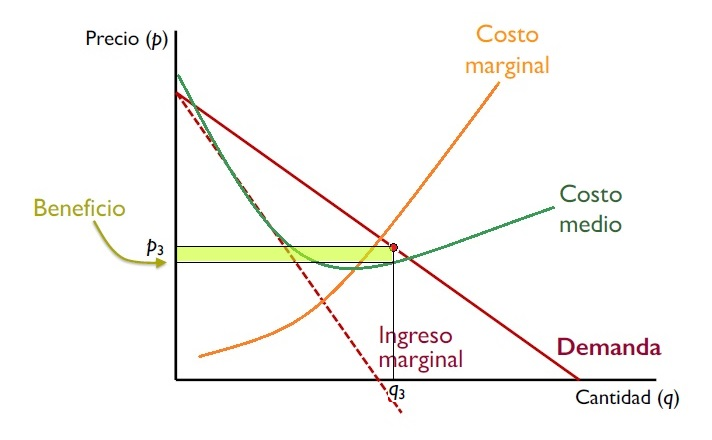
\includegraphics[scale=0.6]{Figures/Tema_06.36_beneficios3.jpg}
\end{frame}

\begin{frame}
\frametitle{ La lógica marginal}
\begin{itemize}
    \item El punto que maximiza el beneficio es donde la curva de IMg cruza la curva de CMg
    \item Recordemos que 
    b = p·q – C(q)
        \begin{itemize}
        \item Para cualquier valor de q, el cambio del beneficio si q fuera aumentado en una unidad sería la diferencia entre el cambio en ingresos, y el cambio en costos: \vspace{2mm} \\ \hspace{10mm}
    Beneficio marginal = IMg - CMg
        \vspace{2mm} \\
        \item Entonces: \\
            - Si $IMg > CMg$ aumentando q se podrían incrementar los beneficios \\
            - Si $IMg < CMg$ el beneficio marginal es negativo, con lo que sería mejor disminuir q para aumentar los beneficios
    \end{itemize}
    \end{itemize}
\end{frame}

%\begin{frame}
%\frametitle{12. De otra forma...}
%\includegraphics[scale=0.6]{Figures/Tema_06.37_diferenciaingresocosto.png}
%\end{frame}

\begin{frame}
\frametitle{ Excedentes y peso muerto}
\begin{itemize}
    \item Las ganancias totales del intercambio están determinadas por los excedentes de consumidores y productores
    \begin{itemize}
        \item El excedente del consumidor \\ - Diferencia entre disposición a pagar y precio de compra
        \item Excedente del productor \\ - Diferencia entre precio y costo de una unidad adicional
    \end{itemize}
    \item Si no terminamos en una asignación Pareto eficiente tenemos una ‘pérdida de peso muerto’
    \begin{itemize}
        \item Pérdida de excedente total con respecto a una asignación eficiente de Pareto \\
        - Es decir, hay ganancias no explotadas del comercio
    \end{itemize}
    \end{itemize}
\end{frame}

\begin{frame}
\frametitle{ Precios y excedentes}
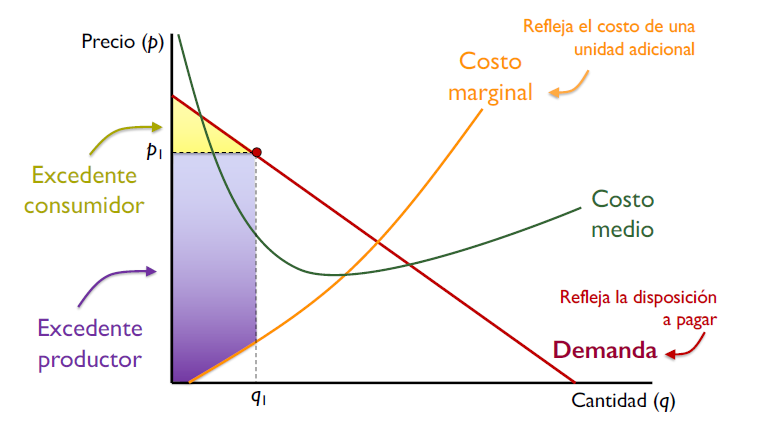
\includegraphics[scale=0.6]{Figures/Tema_06.38_excedente1.png}
\end{frame}

\begin{frame}
\frametitle{Mejora de Pareto}
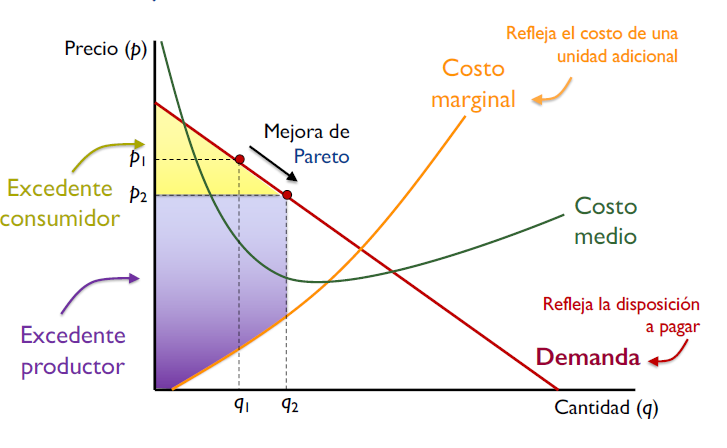
\includegraphics[scale=0.6]{Figures/Tema_06.39_excedente2.png}
\end{frame}

\begin{frame}
\frametitle{Eficiencia de Pareto}
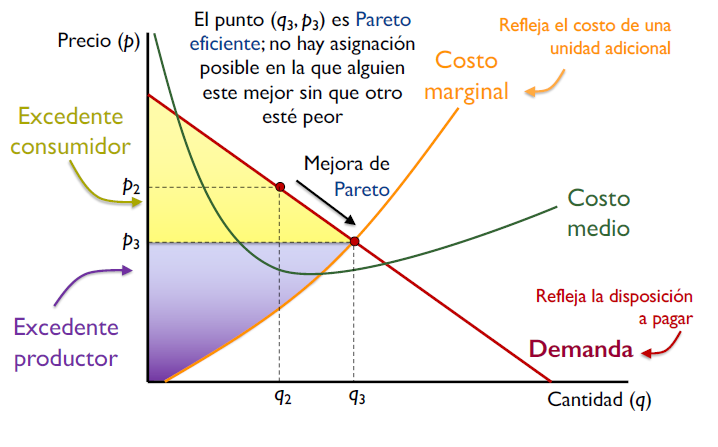
\includegraphics[scale=0.6]{Figures/Tema_06.40_excedente3.png}
\end{frame}

\begin{frame}
\frametitle{Cuando maximiza la firma}
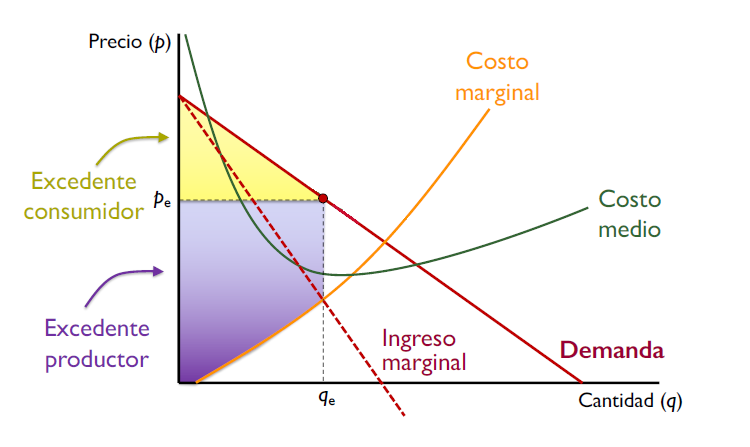
\includegraphics[scale=0.6]{Figures/Tema_06.41_excedente4.png}
\end{frame}

\begin{frame}
\frametitle{ Pérdida de eficiencia}
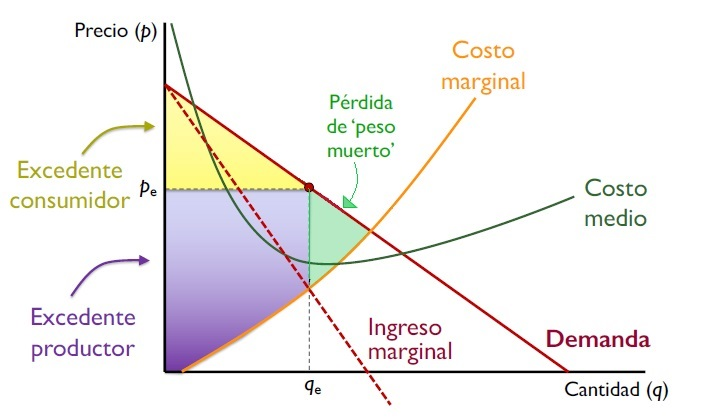
\includegraphics[scale=0.6]{Figures/Tema_06.42_excedente5.jpg}
\end{frame}

\begin{frame}
\frametitle{ Elasticidad y maximización}
\begin{itemize}
    \item Claramente, la firma va a elegir un nivel de producción en la parte elástica de la demanda
    \begin{itemize}
        \item Cuando en la parte inelástica, $IMg < 0$, con lo cual se puede estar mejor reduciendo la producción
    \end{itemize}
    \item La elasticidad precio de la demanda afecta el margen de beneficio $(p – CMg)$ de la empresa
    \begin{itemize}
        \item Cuanto mas elástica es la curva, menos margen, y menor la perdida de peso muerto \\
        - Pequeños cambios en precios $\rightarrow$ gran diferencia en ventas
        \item El markup (margen de ganancia como \% del precio) es inversamente proporcional a la elasticidad precio de la demanda
    \end{itemize}
\end{itemize}
\end{frame}

\begin{frame}
\frametitle{Demanda más elástica}
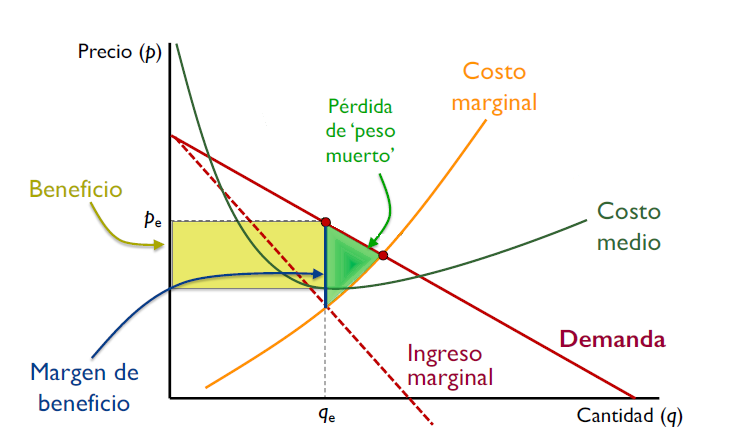
\includegraphics[scale=0.6]{Figures/Tema_06.47_elasticidad3.png}
\end{frame}

\begin{frame}
\frametitle{Demanda más inelástica}
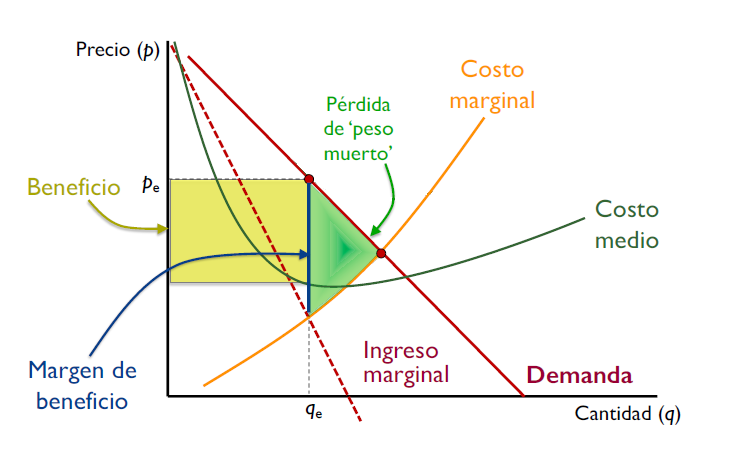
\includegraphics[scale=0.6]{Figures/Tema_06.48_elasticidad4.png}
\end{frame}

\begin{frame}
\frametitle{Poder de mercado}
\begin{itemize}
    \item El margen de beneficio de una empresa depende de la elasticidad de la demanda
    \begin{itemize}
        \item Esta, a su vez se ve afectada por la competencia: \\
        - Demanda relativamente inelástica si hay pocos sustitutos \\
        - Las empresas con poder de mercado tienen suficiente poder de negociación para fijar los precios sin perder clientes a los competidores 
    \end{itemize}
    \item La política de competencia (antitrust), que limita el poder de mercado, puede beneficiar a los consumidores
    \begin{itemize}
        \item Por ejemplo, cuando empresas se pueden agrupar en un cartel (poniéndose de acuerdo para mantener precios altos)
    \end{itemize}
\end{itemize}
\end{frame}

\begin{frame}
\frametitle{ Ganando poder de mercado}
\begin{itemize}
    \item ¿Cómo aumentar el poder de mercado?
    \begin{itemize}
        \item La innovación tecnológica permite diferenciar los productos \\
        - Una empresa que inventan un producto completamente nuevo pueden prevenir la competencia por completo a través de patentes o las leyes de copyright
        \item Con la publicidad las empresas pueden atraer a los consumidores, alejándolos de la competencia y creando lealtad a la marca \\      - Puede ser más eficaz que los descuentos en el aumento de la demanda de una marca
        \end{itemize}
        \item Ambas tácticas pueden cambiar la curva de demanda que enfrenta la empresa
\end{itemize}
\end{frame}

\begin{frame}
\frametitle{Monopolios naturales}
\begin{itemize}
    \item Hay casos en los cuales el poder monopólico surge de características tecnológicas, de estructura de costos
    \begin{itemize}
        \item Cuando el costo medio es decreciente \\
        - Economías de escala, altos costos fijos, o precios de factores que caen cuanto mas compra la empresa
        \item La empresa debe elegir un precio al menos igual al costo medio, que es más alto que el costo marginal \\
        - ¿Por qué?
        \end{itemize}
    \item En estos casos tenemos un monopolio natural
    \begin{itemize}
        \item En estos casos, en lugar de fomentar la competencia, el gobierno suele poner controles de precios o hacer estas empresas de propiedad pública
    \end{itemize}
    \end{itemize}
\end{frame}

\begin{frame}
\frametitle{Casos ideales}
\small
\begin{center}
    \begin{tabular}{c|c}
    \hline
    \hline
    Tomadores de precios & Fijadores de precio \\
    Competencia Perfecta & Monopolio
    \\
    \hline
    \hline
    Puede ser   & Pareto ineficiente \\ 
    Pareto eficiente & (pérdidas peso muerto)
    \\
    \hline
    No hay rentas & Rentas económicas \\
    económicas en & tanto a largo \\
    el largo plazo & como a corto plazo
    \\
    \hline
    Poca gasto en su & Firmas publicitan \\ publicidad & producto único 
    \\
    \hline
    Pocos incentivos para & Firmas invierten en IyD \\ 
    la innovación porque & (tratan de evitar ser \\
    porque otras van a copiar & copiadas)
\end{tabular}
\end{center}
\end{frame}

\begin{frame}
\frametitle{ Competencia imperfecta}
\begin{itemize}
    \item La empresa típica se ubica en algún punto entre los casos extremos de la competencia perfecta y el monopolio \vspace{2mm}
    \item Mercados de competencia imperfecta 
    \begin{itemize}
        \item Oligopolio: sólo hay pocos vendedores, cada uno de los cuales ofrece un producto idéntico o similar a los productos ofrecidos por otros vendedores
        \item Competencia monopolística: existen numerosas empresas que venden productos similares, pero no idénticos porque logran diferenciarse
    \end{itemize}
    \end{itemize}
\end{frame}

\begin{frame}
\frametitle{ Determinantes de la concentración}
\begin{itemize}
    \item Costos
        \begin{itemize}
        \item La existencia de economías de escala hace que solo sobrevivan en el mercado pocas empresas produciendo una gran parte de lo que demanda el mercado 
        \end{itemize}
    \vspace{2mm}
    \item Barreras a la entrada 
        \begin{itemize}
        \item Cuando hay barreras a la entrada se bloquea el acceso para que otros empresas ingresen al mercado
        \end{itemize}
    \vspace{2mm}
    \item Interdependencia estratégica
        \begin{itemize}
        \item Cuando las decisiones de una empresa dependen de las decisiones que toman otras empresas 
        \end{itemize}
    \end{itemize}
\end{frame}

\begin{frame}
\frametitle{Oligopolio}
\begin{itemize}
    \item Competencia entre unas pocas empresas 
    \item Obliga a las empresas a tener en cuenta las reacciones de las competidoras a las desviaciones de los precios de los niveles de producción
    \item Se introducen consideraciones estratégicas en sus mercados
\end{itemize}
\end{frame}

\begin{frame}
\frametitle{ Cartel}
\begin{itemize}
    \item Es una organización de empresas independientes, que producen bienes similares
    \item Trabajan conjuntamente para elevar los precios y restringir la producción
    \item Se comportan como un monopolista
    \item Colusión explicita versus colusión tácita
    \item Ejemplos: DeBeers y OPEP
    \end{itemize}
\end{frame}

\begin{frame}
\frametitle{ La maximización de beneficios del Cartel}
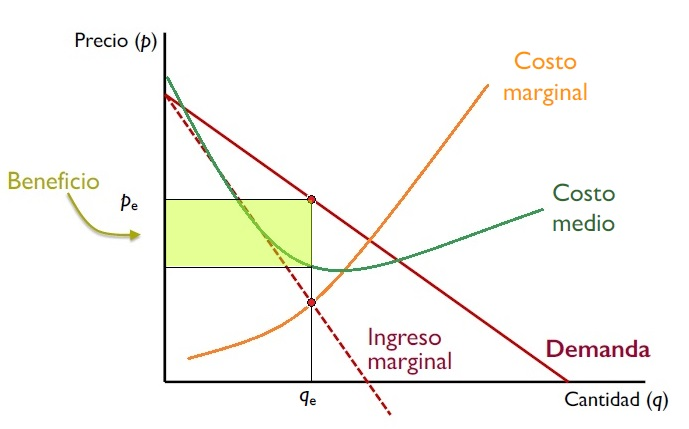
\includegraphics[scale=0.6]{Figures/Tema_06.35_beneficios2.jpg}
\end{frame}

\begin{frame}
\frametitle{Obstáculos para el cartel}
\begin{itemize}
    \item Son ilegales 
    \item Hay incentivos para romper los acuerdos
    \begin{itemize}
        \item Cobrando un precio apenas más bajo, una empresa aumentando su participación de mercado y saca enormes beneficios
        \item Esto sucede porque la demanda es elástica
    \end{itemize}
    \item Hoy en día hay una fuerte competencia procedente de empresas extranjeras además de las nacionales
\end{itemize}
\end{frame}

\begin{frame}
\frametitle{ ¿Cómo compiten pocas empresas?}
\begin{itemize}
    \item Competencia por cantidades \vspace{1mm}
    \item Competencia por precio  \vspace{1mm}
    \item Líder y seguidores 
\end{itemize}
\end{frame}

\begin{frame}
\frametitle{ Competencia monopolística}
\begin{itemize}
    \item Hay muchos compradores y vendedores
    \item Es fácil entrar y salir
    \item Las empresas toman los precios de las demás como los proporcionan
    \item Los productos están diferenciados
    \begin{itemize}
        \item Cada vendedor tiene libertad para subir o bajar los precios debido a la diferenciación de productos
        \item Entonces, la curva de demanda de cada vendedor tenga pendiente negativa
    \end{itemize}
    \end{itemize}
\end{frame}

\begin{frame}
\frametitle{ La maximización de beneficios en Competencia Monopolística en corto plazo}
\centering
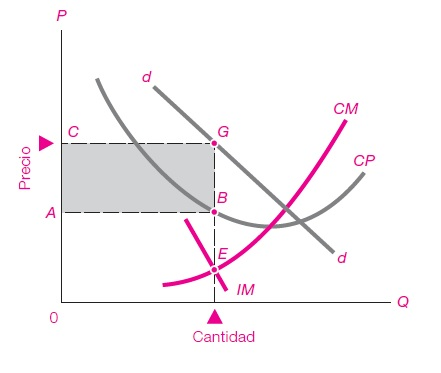
\includegraphics[scale=0.75]{Figures/Tema_08.01_compmonop.jpg}
\end{frame}

\begin{frame}
\frametitle{ Competencia monopolística en el largo plazo}
\begin{itemize}
    \item Los beneficios positivos en el corto plazo atraen nuevas empresas
    \item La demanda que enfrenta la empresa se contrae
    \item Los precios son superiores a los costos marginales
    \item En el largo plazo, los beneficios de la empresa son iguales a cero, es decir, tiene beneficios normales 
\end{itemize}
\end{frame}

\begin{frame}
\frametitle{ La maximización de beneficios en Competencia Monopolística en largo plazo}
\centering
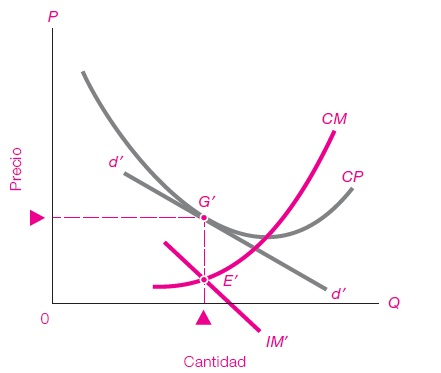
\includegraphics[scale=0.7]{Figures/Tema_08.02_compmonop.jpg}
\end{frame}
\end{document}
